\documentclass[letterpaper]{article}

%% Language and font encodings
\usepackage[english]{babel}
\usepackage[utf8x]{inputenc}
\usepackage[T1]{fontenc}

%% Sets page size and margins
\usepackage[letterpaper,top=3cm,bottom=2cm,left=2cm,right=2cm,marginparwidth=1.75cm]{geometry}

%% Useful packages
\usepackage{amsmath}
\usepackage{graphicx}
\usepackage[colorinlistoftodos]{todonotes}
\usepackage[colorlinks=true, allcolors=blue]{hyperref}

\usepackage[numbered,framed]{matlab-prettifier}
\let\ph\mlplaceholder % shorter macro
\lstMakeShortInline"

\lstset{
  style              = Matlab-editor,
  basicstyle         = \mlttfamily,
  escapechar         = ",
  mlshowsectionrules = true,
}

\title{EE576 HW 4}
\author{Jordan Caudill and Matt Ruffner}

\begin{document}
\maketitle

%%%%%%%%%%%%%%%%%%%%%%%%%%%%%%%%%%%%%%%%%%%%%%%%%%%%%%%%%%%%%%%%%%
%%%%%%%%%%%%%%%%%%%%%%%%%%%%%%%%%%%%%%%%%%%%%%%%%%%%%%%%%%%%%%%%%%
%%%%%%%%%%%%%%%%%%%%%%%%%%%%%%%%%%%%%%%%%%%%%%%%%%%%%%%%%%%%%%%%%%
\section{}
Their rational is not valid. Like the Stuxnet attach, the 'air gap' is able to be bridged by means of inserting a flash drive into the target computer. Even though the computer is not connected to the internet, any malicious actor within the known operating staff of the damn would be able to initiate a malicious attach. There is also the scenario of someone sneaking past security in order to initiate the attack. These are two reasons that the penalty incurred by shutting down the equipment for several hours is less than the possibility of malicious acting.


%%%%%%%%%%%%%%%%%%%%%%%%%%%%%%%%%%%%%%%%%%%%%%%%%%%%%%%%%%%%%%%%%%
%%%%%%%%%%%%%%%%%%%%%%%%%%%%%%%%%%%%%%%%%%%%%%%%%%%%%%%%%%%%%%%%%%
%%%%%%%%%%%%%%%%%%%%%%%%%%%%%%%%%%%%%%%%%%%%%%%%%%%%%%%%%%%%%%%%%%
\section{}
We begin by defining normal accidents as incidents that were due to unforeseeable circumstances. Based on this definition we can analyze the following situations: 
\\
\\
a. The Stuxnet attack is not an example of a normal accident. This is because is was an intentional, malicious attack designed to cause as much damage as possible. It was caused by a usb stick containing the virus being placed in a target computer through either infiltration or social engineering. This resulted in significant damage to Iran's nuclear program. The way to prevent this would be to have more security or training of personal. Because it was a malicious attack that could have been predicated and avoided it is not a normal accident.
\\
\\
b. The ruptured pipeline in Bellingham, Washington is an example of a normal accident. The accident was caused due to a faulty computer SCADA system and faulty pressure valve. Because the failure was due to faulty equipment and not a malicious attack, it could not have been predicted. This is why it is an example of a normal accident.
\\
\\
c. The hijacked trams in Lodz, Poland was not a normal accident. This is because it was caused by a teen who used an electric remote to change the railway connections causing multiple injuries. He was able to do this because he trespassed into the train depots to gather information he needed. This could have been avoided with better security and a more secure system. Because of that, it is not a normal accident.
\\
\\
d. The 2011 failure at the Illinois water plant is not an example of a normal accident. While it was initially considered to be caused by Russian hackers, it was later revealed to be cause by a faulty pump. The confusion was caused when a contractor with remote access to the pump signed on while he was on vacation in Russia. The pump had been experiencing problems for a while so it should have been changed. Because they had experienced problems before, they should have known that it would fail eventually. Because they could have predicted it, it is not a normal accident. 



%%%%%%%%%%%%%%%%%%%%%%%%%%%%%%%%%%%%%%%%%%%%%%%%%%%%%%%%%%%%%%%%%%
%%%%%%%%%%%%%%%%%%%%%%%%%%%%%%%%%%%%%%%%%%%%%%%%%%%%%%%%%%%%%%%%%%
%%%%%%%%%%%%%%%%%%%%%%%%%%%%%%%%%%%%%%%%%%%%%%%%%%%%%%%%%%%%%%%%%%
\section{}
The appeal to attacking smart meters lies in the fact that it is possible to obtain private information about the household with which they are attach. This is done by monitoring the "energy consumption traces"~\cite{RajagopalanS.R2011SmpA}. By using frequent meter readings combined with data mining algorithms, it is possible to obtain private information about the occupant of the home~\cite{RajagopalanS.R2011SmpA}. The information that can be obtained include: number of occupants, life-style and economic status, and with fine enough measurements they could even monitor which channel on television is being watched. Because the smart meter is designed to be used in real time with the smart grid, all this information would be available to an attacker in real time. 



%%%%%%%%%%%%%%%%%%%%%%%%%%%%%%%%%%%%%%%%%%%%%%%%%%%%%%%%%%%%%%%%%%
%%%%%%%%%%%%%%%%%%%%%%%%%%%%%%%%%%%%%%%%%%%%%%%%%%%%%%%%%%%%%%%%%%
%%%%%%%%%%%%%%%%%%%%%%%%%%%%%%%%%%%%%%%%%%%%%%%%%%%%%%%%%%%%%%%%%%
\section{}

\paragraph{a.}

DPA or Differential Power Analysis is the act of measuring the different voltage or current that happens during the encryption process to try to obtain the hidden key. This is done in the following steps:
\begin{enumerate}
    \item Find an intermediate value of $v_{i,k}=f(d_{i},k)$. This means that you take a value to be encrypted and run it through the encryption hardware, where $v_{i,k}$ is the voltage, $d_{i}$ is the data point and k is the key.
    
    \item  Measure the power traces at $t_{i,k}$ while encrypting $d_{i}$. This means to measure a particular power trace at a given time while encrypting the data.
    
    \item  Build a matrix of all the hypothetical intermediate values inside the cipher for all possible keys and $v_{i,k}$ traces. This means building a matrix that could contains all the possible voltage values from step 1 in the columns and have it with all the possible keys in the rows.
    
    \item Build a matrix of all the hypothetical power consumption values and all possible keys. This means building a matrix with what we predict the power to be in the columns ($h_{i,k}$) with the possible keys in the rows.
    
    \item Statistically evaluate which key hypothesis best matches the measured power at each individual time. This is done by using the correlation function with the matrices from steps 3 and 4 and find the max value of the new matrix. This has the highest chance of being the key.
\end{enumerate}


\paragraph{b.}
Code from \texttt{measurement.m} is shown in Listing \ref{meas} and code from \texttt{mycorr.m} is shown in Listing \ref{mycorr}.

\lstinputlisting[language=Matlab,caption={\texttt{mycorr.m} code},label={mycorr}]{mycorr.m}

\lstinputlisting[language=Matlab,caption={\texttt{measurement.m} code},label={meas}]{measurement.m}



\newpage
\paragraph{c.}

The unknown key was determined to be:

\vspace{1cm}
\textbf{\texttt{
0x05 
0xDE 
0xAD 
0xBE 
0xEF
0x42
0x00
0x68
0x61
0x63
0x6B
0x65
0x64
0x6B
0x65
0x79}}\\
\vspace{1cm}\\
The plot in Fig. \ref{fig:traceIndex} shows the points along the mean of the power traces where the correct key was located during the examination of the correlation matrix. As you can see, the correct keys were found relatively early on within the entire power monitoring trace, indicating that less samples could have sufficed in order to still successfully glean the 16 byte key from the trace.

In Fig. \ref{fig:traceIndex}, you can see the low portions within the raised portion of the signal. These represent the 10 rounds of encryption. The estimates yeilded by the correlation power analysis (differential power analysis) are accurate enough to extract the key without power trace data on all rounds of AES encryption.

\begin{figure}[h!]
\centering
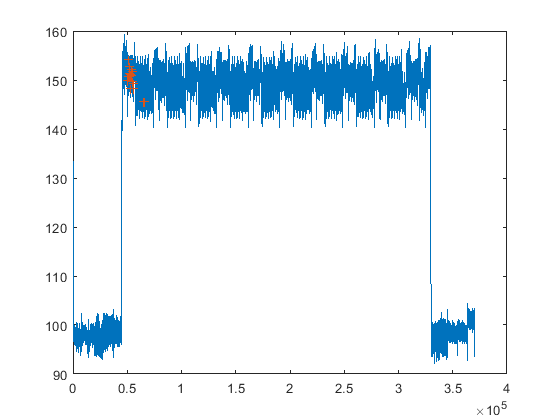
\includegraphics[width=10cm]{keyIndexPlot.png}
\caption{Plot showing the trace indices corresponding to the correct key}
\label{fig:traceIndex}
\end{figure}

\paragraph{d.}
It was interesting how little of the entire collected traces was actually needed to successfully determine the key. One challenge faced was calculating the bitwise hamming distance in MATLAB. In looking at other implementations of this code, specifically Phillip's~\cite{gaphil}, we have implemented a much faster search of the correlation matrix in order to find the correct corresponding key and time within the trace using the line \texttt{[K,T]=find(CC==max(max(CC)));} instead of manually iterating.


%%%%%%%%%%%%%%%%%%%%%%%%%%%%%%%%%%%%%%%%%%%%%%%%%%%%%%%%%%%%%%%%%%
%%%%%%%%%%%%%%%%%%%%%%%%%%%%%%%%%%%%%%%%%%%%%%%%%%%%%%%%%%%%%%%%%%
%%%%%%%%%%%%%%%%%%%%%%%%%%%%%%%%%%%%%%%%%%%%%%%%%%%%%%%%%%%%%%%%%%
\bibliographystyle{ieeetr}
\bibliography{refs.bib}

\end{document}